%\documentclass[handout]{beamer}
%\documentclass[14pt]{beamer}
\documentclass{beamer}

\usepackage[english]{babel}
\usepackage[utf8]{inputenc}
\usepackage{multirow}
\usepackage{booktabs}
\usepackage{amsmath}
\usepackage{amssymb}
\usepackage{subfigure}
\usepackage{color}
\usepackage{graphicx}
\definecolor{blue}{RGB}{000, 103, 198}
\definecolor{green}{HTML}{249140}
\definecolor{red}{HTML}{c71712}
\usepackage{colortbl}
\usepackage{tikz}
\usepackage{pgfplots}
\pgfplotsset{compat=1.5.1}

\bibliographystyle{apalike}

\usetikzlibrary{decorations.pathreplacing}
\usetikzlibrary{intersections}
\usetikzlibrary{shapes,snakes}

\usecolortheme[RGB={000, 103, 198}]{structure}
\setbeamertemplate{footline}[frame number]
\setbeamertemplate{navigation symbols}{}

\colorlet{darkgreen}{green}
\colorlet{darkred}{red}

\renewcommand<>{\alert}[1]{{\color#2{darkred}#1}}
\newcommand<>{\alertg}[1]{{\color#2{darkgreen}#1}}
\newcommand<>{\alertb}[1]{{\color#2{blue}#1}}

\title{ARCH-COMP Category Report:\\ Continuous and Hybrid Systems with 
Nonlinear Dynamics}

\author{
  Fabian Immler,
  Matthias Althoff,
  Xin Chen,
  Chuchu Fan,
  Goran Frehse,
  %  Ariful Islam
  %  \and 
  Niklas Kochdumper,
  Yangge Li,
  Sayan Mitra,
  Mahendra Singh Tomar,
  Majid Zamani
}
\institute{
  Technische Universit\"at M\"unchen (Germany), University of Dayton (USA), 
  University of Illinois at Urbana-Champaign (USA),
  Univ. Grenoble Alpes (France)
}
\AtBeginSection[]{
  \begin{frame}
  \vfill
  \centering
  \begin{beamercolorbox}[sep=8pt,center,shadow=true,rounded=true]{title}
    \usebeamerfont{title}\insertsectionhead\par%
  \end{beamercolorbox}
  \vfill
\end{frame}
}

\begin{document}

\frame{\thispagestyle{empty}\titlepage}

\section{Tools}

\begin{frame}{Tools I}

\begin{itemize}
  \item \textbf{CORA}: zonotopes, linearization / polynomial zonotopes
  \item \textbf{CORA/SX}: basic zonotope reachability  algorithm of CORA, 
    ported to SpaceEx
  \item \textbf{SymReach}: basic zonotope reachability  algorithm of CORA,
    implemented in C++
\end{itemize}

\end{frame}


\begin{frame}{Tools II}

\begin{itemize}
  \item \textbf{C2E2}: simulation, on-the-fly discrepancy computation for neighboring trajectories
  \item \textbf{Flow*}:\\
    continuous reachability: Taylor Models, symbolic remainders \\
    discrete jumps: domain contraction, range overapproximation, box/parallelotope aggregation
  \item \textbf{Isabelle/HOL}: formally verified (performance secondary) \\
	zonotopes, affine arithmetic, Runge-Kutta methods
\end{itemize}
\end{frame}


\section{Benchmarks}

\begin{frame}{Benchmarks}
\begin{itemize}
	\item three (continuous) from last year
	\item one (hybrid) new
\end{itemize}
\end{frame}

\begin{frame}{van-der Pol (2-dimensional)}
\begin{itemize}
	\item pseudo invariant $x = 1.5$ \\ (CORA,CORA/SX,Isabelle/HOL): 0.6 - 2.3 s
	\item without pseudo invariant: \\
		1.5 s (Flow*), 40 s (C2E2), 17 s (SymReach)
\end{itemize}
\begin{figure}[p]
	\centering
	\subfigure[CORA/SX] 
	{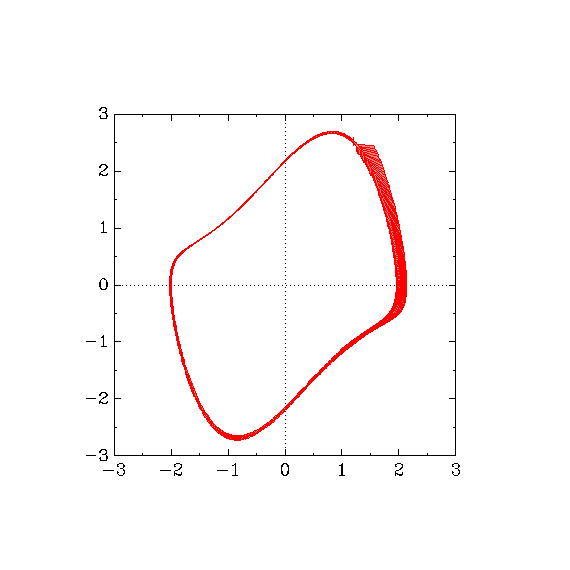
\includegraphics[width=5cm, height=5cm, trim=50 50 50 50, clip=true]{../results_SpaceEx/vdp-zono.png}}
	\subfigure[SymReach]{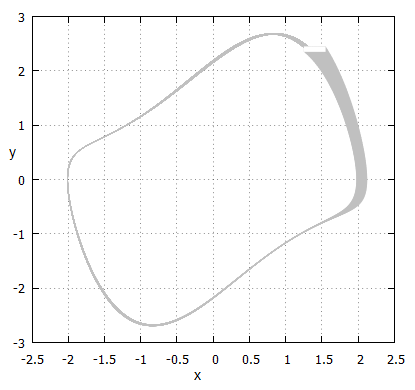
\includegraphics[width=5cm, height=5cm]{../results_SymReach/vanderpol.png}}
\end{figure}
\end{frame}

\begin{frame}{Laub-Loomis (7-dimensional)}
\begin{itemize}
  \item challenge: larger initial set, therefore\\
  	larger non-convex reachable sets
  \item only CORA (polynomial zonotope), C2E2 (simulation), and Flow* (Taylor models) can handle larger initial set
\end{itemize}
\begin{figure}[p]
	\centering
	\subfigure[CORA/SX (small initial set)] 
	{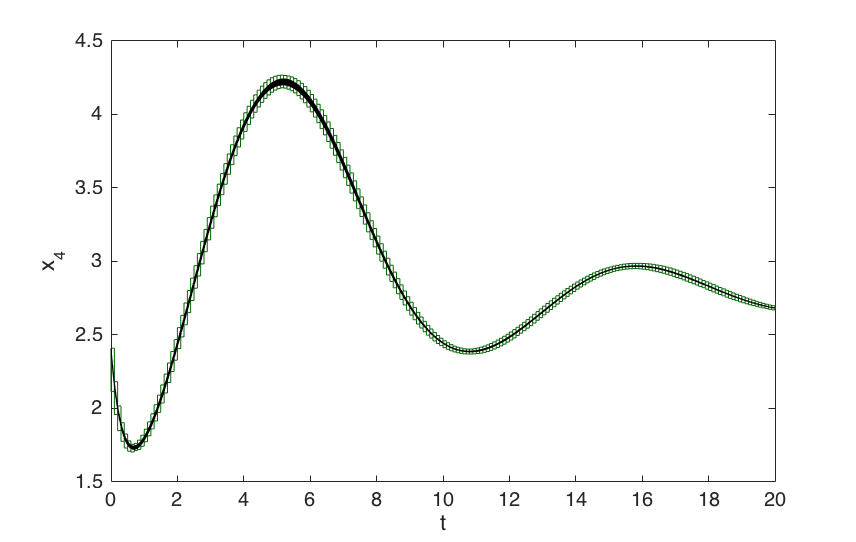
\includegraphics[width=5cm, height=5cm]{../results_flowstar/laub_loomis_small.png}}
	\subfigure[SymReach (large initial set)]{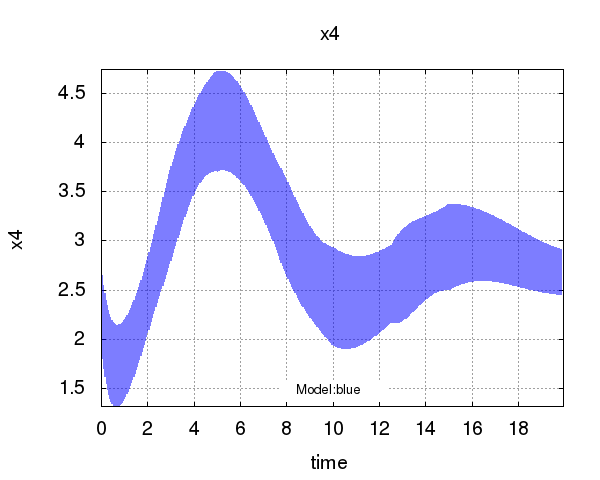
\includegraphics[width=5cm, height=5cm]{../results_C2E2/laub_large.png}}
\end{figure}
\end{frame}

%\begin{frame}
%\begin{table}[t]
%\setlength{\tabcolsep}{4pt}
%\renewcommand{\arraystretch}{1.2}
%\centering
%\caption{Results of the Laub-Loomis model.}
%\begin{tabular}[c]{lcc}
%	\hline
%	& \multicolumn{2}{c}{\textbf{computation time in [s]}}\\ \cmidrule(l){2-3}
%	\textbf{tool} & \textbf{$W=0.01$} & \textbf{$W=0.1$} \\ \hline
%	CORA & $0.82$ & $63$ \\
%	CORA/SX & $0.85$ & -- \\
%	C2E2 & {$0.12$} & {$0.67$} \\
%	Flow* & $4.5$ & $12.7$ \\
%	Isabelle/HOL & $10$ & $-$ \\
%	SymReach & $1.93$ & $-$ \\
%	\hline
%\end{tabular}
%\label{tab:compTimes:laubloomis}
%\end{table}
%\end{frame}

\begin{frame}{Quadrotor (7-dimensional)}
\begin{figure}
	\subfigure[Isabelle/HOL]{
	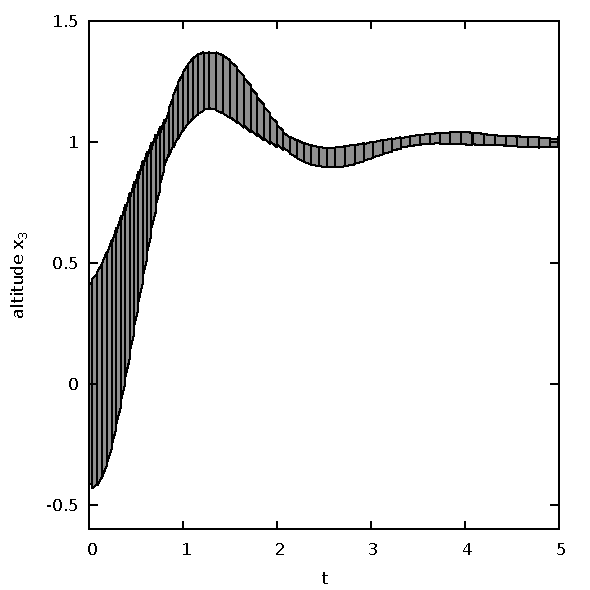
\includegraphics[width=4cm, height=4cm]{../results_Isabelle/out_quadrot.pdf}}
	\subfigure[all tools performing well]{\small
		\begin{tabular}[c]{lc}
			\hline
			\textbf{tool} & \textbf{computation time in [s]} \\
			\hline
			CORA & $5.2$\\
			CORA/SX & $1.5$ \\
			Flow* & $5.9$ \\
			Isabelle/HOL & 30 \\
			SymReach & 2.96 \\
			\hline
		\end{tabular}
	}
\end{figure}
\end{frame}

\begin{frame}{Space Rendezvous (4-dimensional, hybrid)}

	\begin{itemize}
		\item nonlinear version of linearized Space Rendezvous in ARCH-COMP ``Linear''
		\item not very challenging \\ (provided \emph{some} means to compute discrete jumps)
	\end{itemize}
	\begin{figure}
		\subfigure[CORA]{
			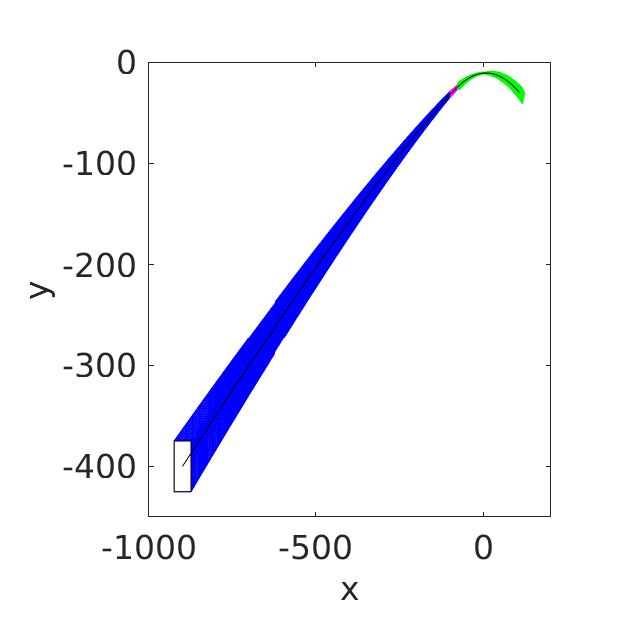
\includegraphics[width=4cm, height=4cm]{../results_CORA/spacecraftNonlin_04June2018.eps}}
		\subfigure{
			\tiny
			\raisebox{9em}{
				\begin{tabular}[c]{lccc}
					\hline
					\textbf{tool} & \textbf{computation time in [s]} \\
					\hline
					CORA & $14.8$ \\
					{C2E2} & {$29.18$} \\
					Flow* & $18.7$ & \\
					Isabelle/HOL & 395 \\
					\hline
				\end{tabular}
			}
		}
	\end{figure}

\end{frame}

\begin{frame}{Conclusions}
\begin{itemize}
  \item doubled number of tools!
  \item One more benchmark (hybrid).
  \item CORA ports: up to 4 times faster, sometimes slower (less algorithms)
  \item Isabelle/HOL: solves more benchmarks than 2017
    (implementation of sin/cos in affine arithmetic)
  \item Flow*: overall performance improvements, C++ API, support analysis of neural network controllers
  \item C2E2: announced new version from the experience of this competition (``results [...] are not optimal'')
\end{itemize}
\end{frame}
\end{document}
